\section{Test and Evaluation}

The requirement of this project is to perform drawing task within position error 10\% range and able to do force control. RMSE (Root Mean Square Error) statistic method can be used to determine the average position error occurs on the system when UR5 done drawing task. With RMSE calculation code, Computer can average the RMSE of each joint over time while UR5 is operated drawing task and when UR5 is done drawing task. \textbf{The average position RMSE of this control system are 0.0022 radian or 1.9\% error from joint limit}. The result of the controller can be seen as drawing in Fig.\ref{fig:drawing}

\begin{figure}[ht]
    \centering
    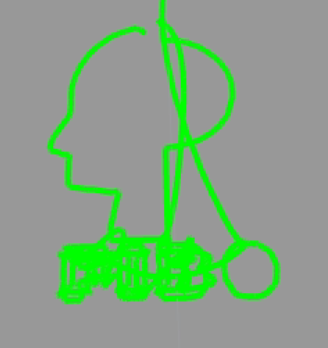
\includegraphics[width=10cm]{img/drawing.png}
    \caption{drawing}
    \label{fig:drawing}
\end{figure}

\vspace{3mm}
The force at the end effector can be achieving desire force and can maintain the force while UR5e perform drawing task as show in Fig.\ref{fig:wrench}. After several tests the force elevation controller unable to perform more that desire z-axis force at -1 N (while end-effector is not touching floor, The force at end-effector is around -3.5 N). After crossing the -1 N boundary, The UR5e can't stabilize the end-effector orientation anymore as show in Fig.\ref{fig:wrench_at_zero}.

\begin{figure}[ht]
    \centering
    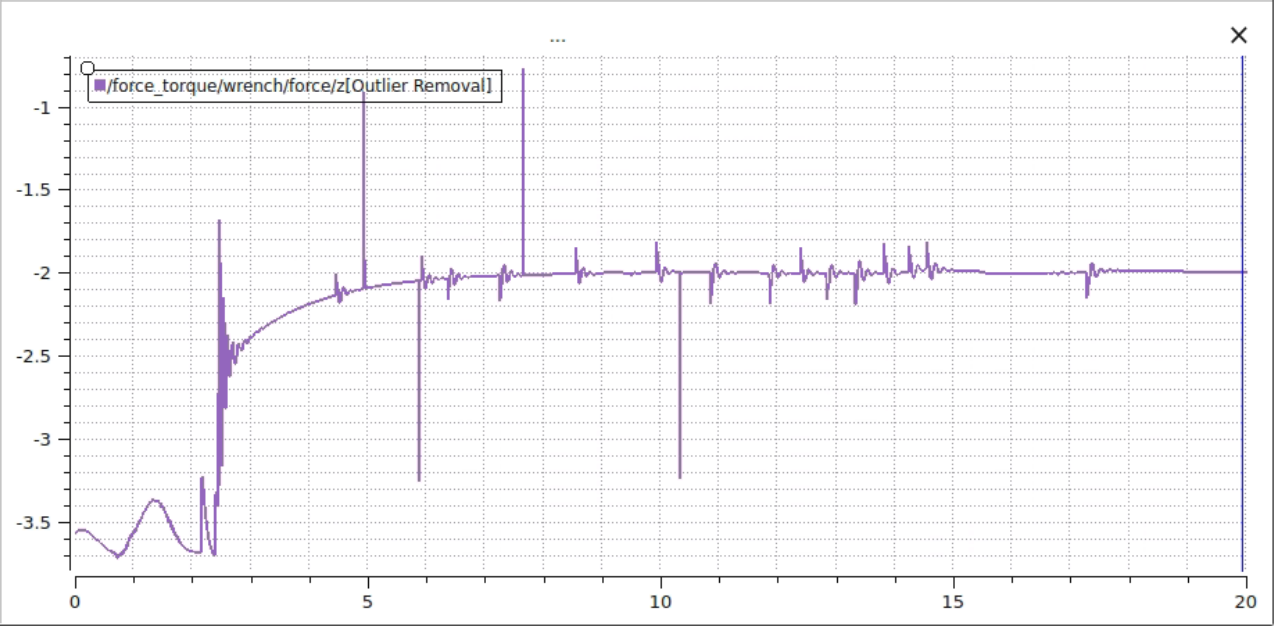
\includegraphics[width=14cm]{img/wrench.png}
    \caption{z-axis end-effector force at desire -2 N while UR5e perform drawing task}
    \label{fig:wrench}
\end{figure}

\begin{figure}[ht]
    \centering
    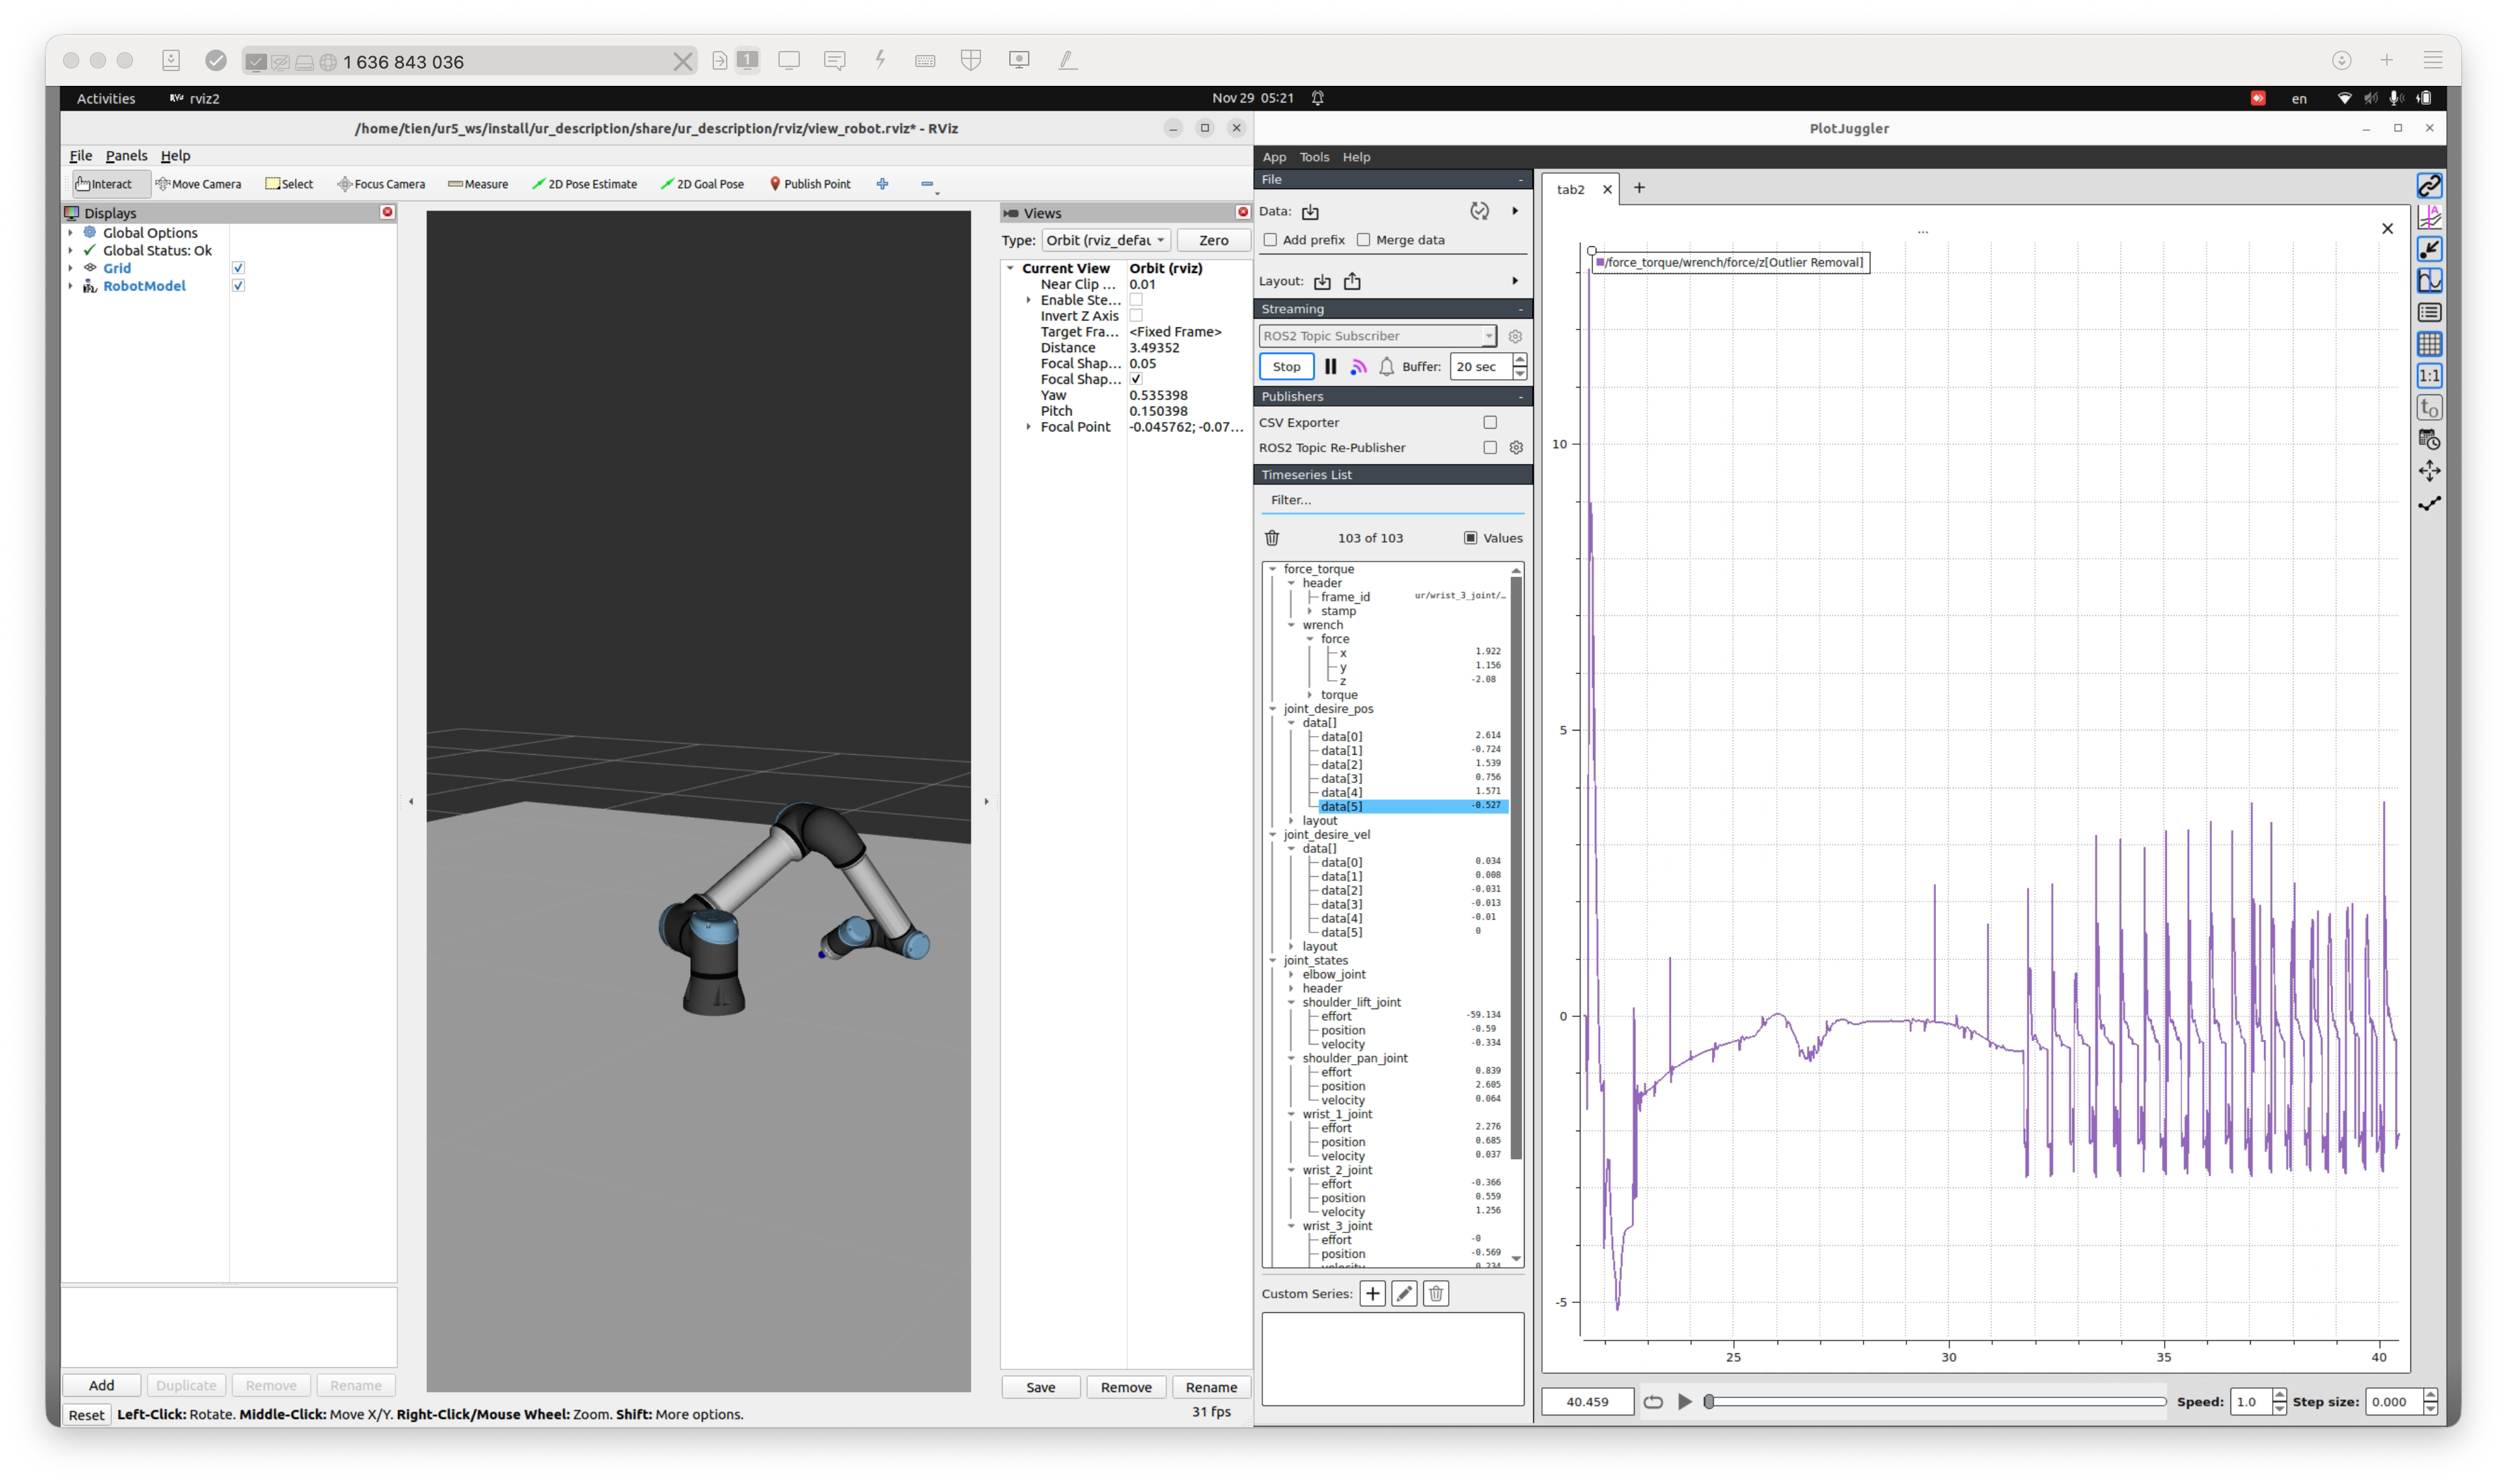
\includegraphics[width=14cm]{img/Wrench0.png}
    \caption{z-axis end-effector force at desire 0 N while UR5e perform drawing task}
    \label{fig:wrench_at_zero}
\end{figure}
